\section{Measurement}
\label{sec:Measurement}

There are several experiments for searching LLPs. MATHUSLA (\atlas), MilliQan (\cms), SHiP. 
But these experiments are so large to compare with CODEX-b, this is a one attractive of CODEX-b. 
We can control backgrounds because it will be placed underground and shields are existed. 
Additional passive Pb shield to suppress muon and neutral hadrons. 
Thin active veto for secondaries inside the shield. 

\begin{figure}[h]
\centering
    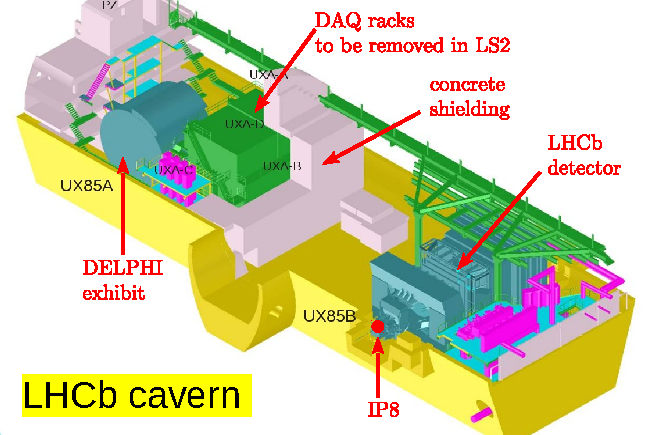
\includegraphics[width=12cm]{figs/INT/lhcb_cavern.pdf}
    \vspace{0.15cm}
\caption{ 
   Schematic plot of LHCb cavern 
}
\end{figure}

\subsection{Compact Detector for Exotics at LHCb}

The Compact Detector for Exotics at \lhcb (CODEX-b) was proposed to observe weakly coupled \textbf{LLP}s in \lhcb cavern. 
Since \atlas and \cms focused on high \pt and large QCD backgrounds and restricted lifetime of \lhcb, current detectors can miss signals from weakly coupled \textbf{LLP}s. 
The size of CODEX-b is 10 X 10 X 10 m shielded box. It is placed 25 m from IP8. 
If \delphi is removed, access to 20 X 10 X 10 m box. 
The CODEX-b consists of two parts. 
6 RPC layers at 4\cm intervals on each box face with 1\cm granularity (Attach the geometry plot of CODEX-b here!!). 
5 equally spaced triplets along the depth to minimize distance between reconstructed vertex and 1st measurement. 
50 - 100 ps timing from RPC's foreseenfor mass reconstruction.

\subsection{Background measurement}

Using two 30 X 30 X 2\cm wrapped plastic scintillators with photomultiplier tube (PMT) attached on iron test stand. 
Each PMTs receives 1.5 kV high voltage and 350 V bias voltage. 
Why do we set high voltage to 1.5 kV? Because rate increases with bigger high voltage, but it becomes flat when high voltage larger than 1.5 kV
The scintillators measure mininum ionizing particles (mip).
This supports by NIM crate.
We test this equipments at lab taking cosimc rays
This is the first time measured hit rate at underground cavern.
Results from measurments may impact to other LLP experiments.
When particle goes through scintillators and makes hits on both detectors, we counts number of events. 
We made 30 mV threshold of signal pick to measure data which has physical meaning. 
Triggering when signals appear at both detector in 5 ns. 
Since detector have been placed 100 m below underground, muons from cosmic rays decay are suppressed. 
We take data during MD and when the beam is online. 
We switch the detector position several times. Also we take data while detector is rotated. 
This is the first measurement of hit rate at D3 platform. 
We use scope to take data, hit rate is not high. 
We remotely connect to scope and able to manage scope.
We took data from 4 different places. 
Back of D3 platform of each corner and central position.
Front D3 platform at central with parallel to beam line and make 45 degree with a beam line.

\begin{figure}[h]
\centering
    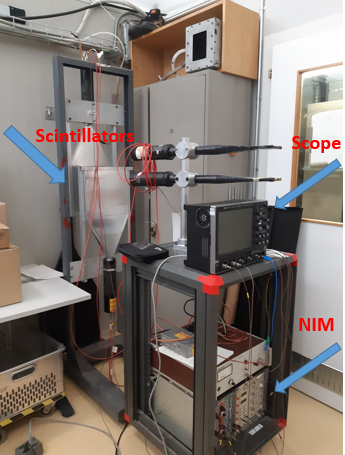
\includegraphics[width=6cm]{figs/INT/Tools.png} 
\caption{ 
    Test-bench photo
}
\end{figure}

\begin{figure}
\centering
    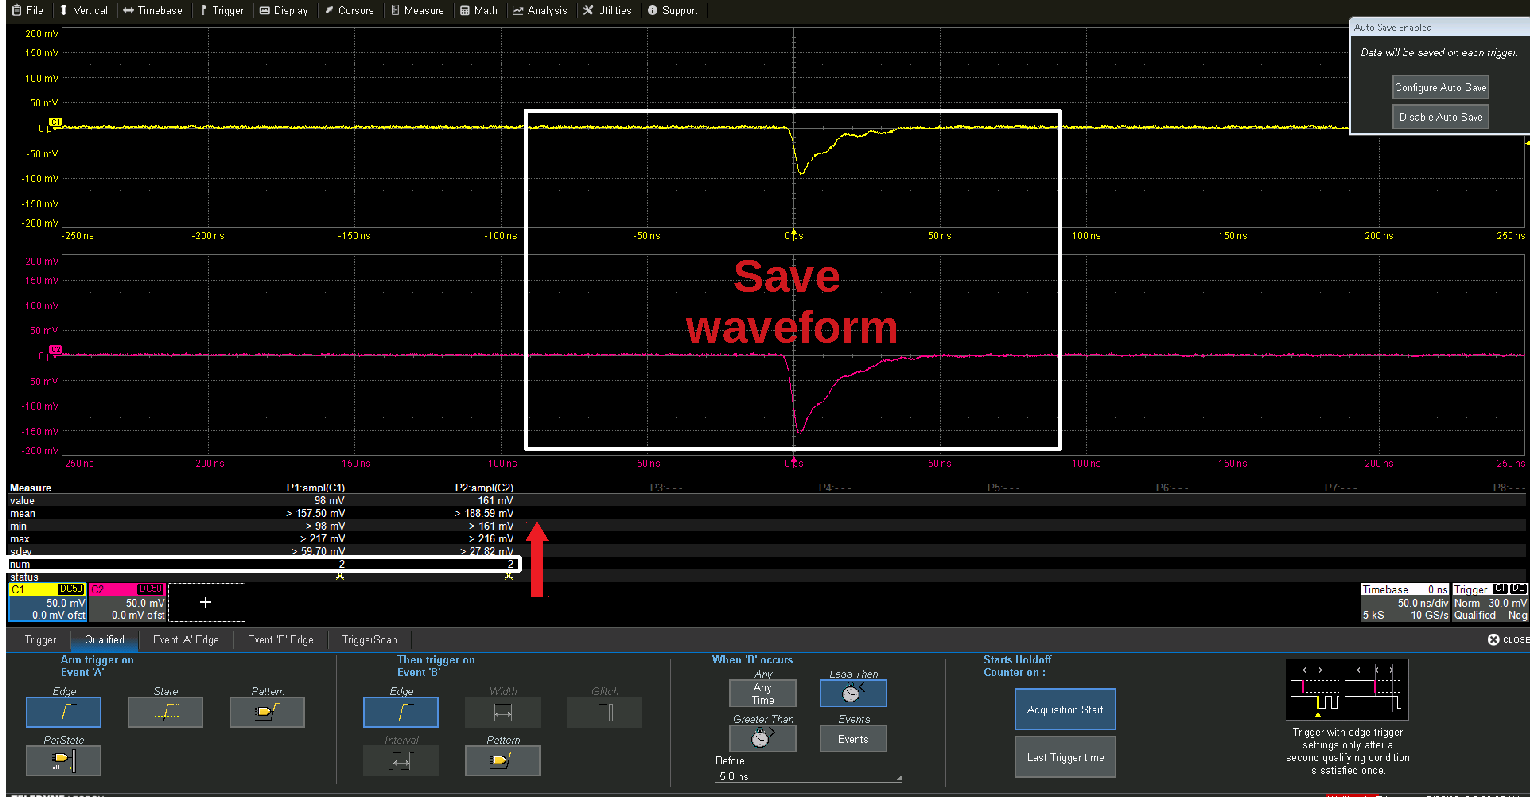
\includegraphics[width=12cm]{figs/INT/waveform.pdf}
\caption{
    Trigger setup
}

\begin{figure}[h]
\centering
    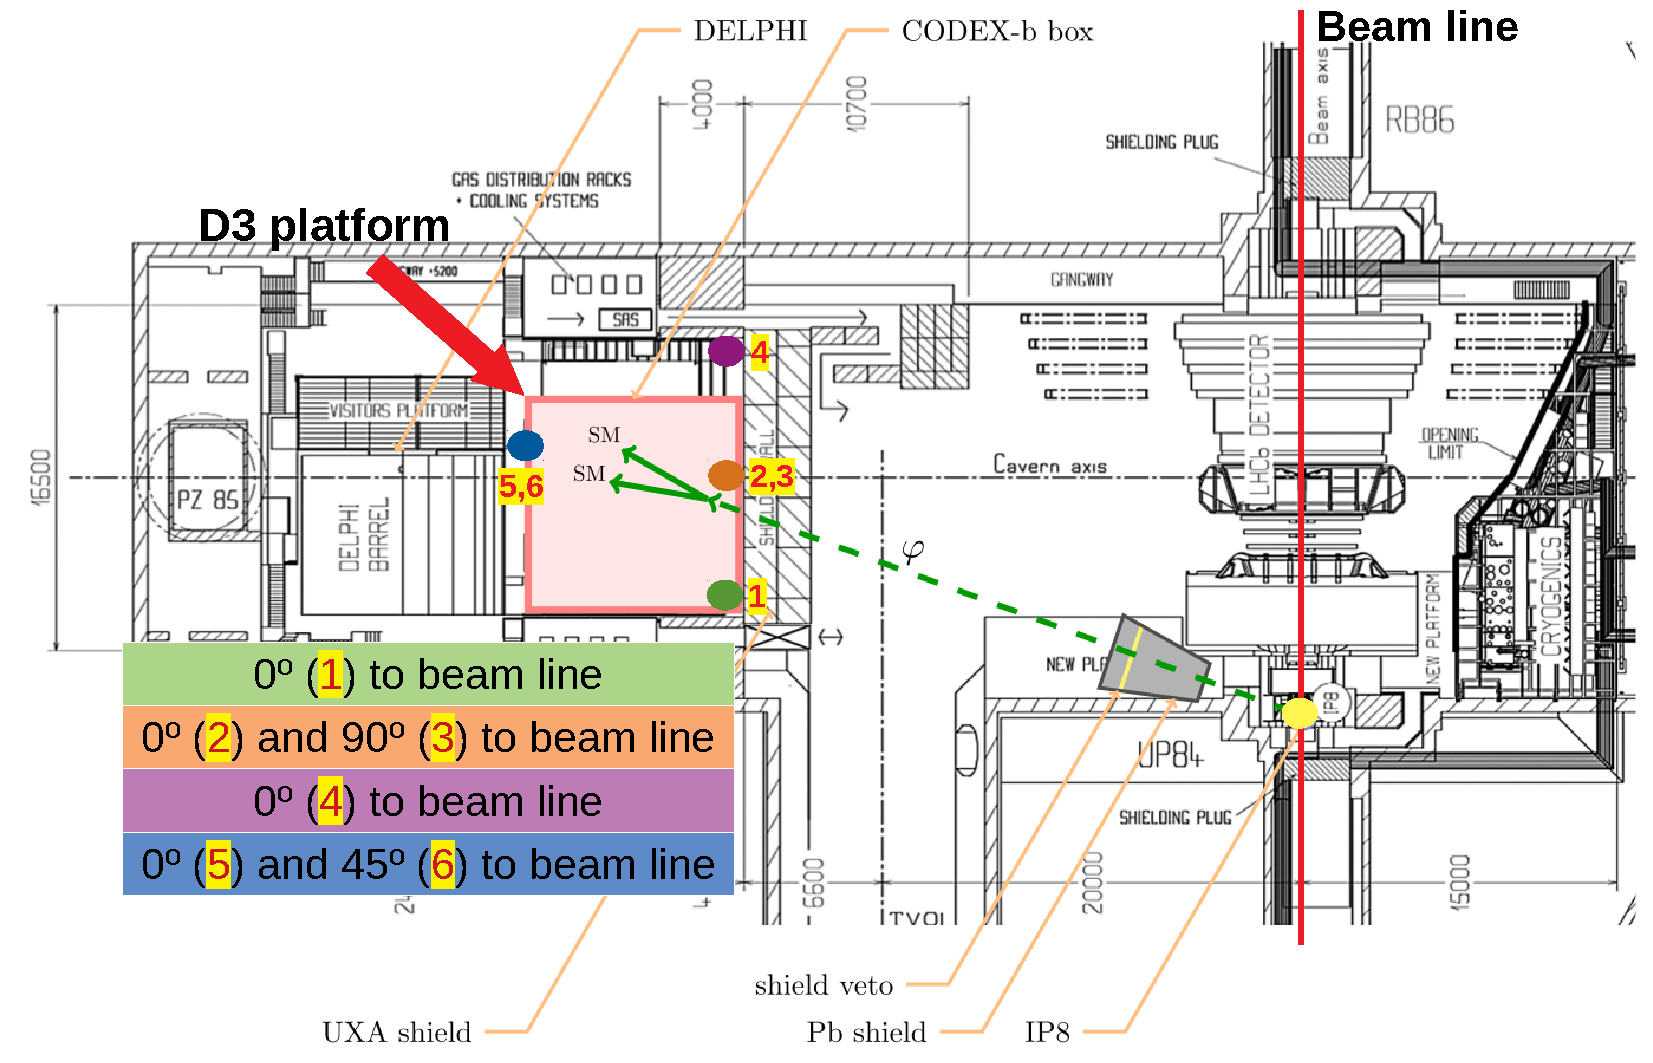
\includegraphics[width=12cm]{figs/INT/configuration.pdf}
\caption{
    Four measurement positions at the LHCb cavern
}
\end{figure}

\subsection{Test-bench}
We used Herschel detector.
For PMT, model: R1828-01
Because, it has high anode current upper limit, wide range of gain variation, fast time response to fit in 25 ns, large entry window to increase light yield, good single electron separation.
The test-bench includes cosmic stand, scope with extended functions (auto save waveforms, coincidence logic), high voltage power supplies (1.5 kV, bias 350 V), current-voltage meter, laptop to remote connect to scope.

\subsection{Trigger}
Simple 2x fold coincidence. 
Distance between two scintillators 2\cm. 
Discrimination (scope) threshold 30 mV.
When first scintillator receive a signal and the other scintillator also receives a signal in 5 ns, scope counts.


